%%%%%%%%%%%%%%%%%%%%%%%%%%%%%%%%%%%%%%%%%%%%%%%%%%%%%%%%
% Este é um documento que servirá de modelo para
% os relatórios feitos na disciplina Circuitos Digitais
% 2016-2
%%%%%%%%%%%%%%%%%%%%%%%%%%%%%%%%%%%%%%%%%%%%%%%%%%%%%%%%%

\PassOptionsToPackage{brazil,american}{babel}
\documentclass[12pt]{article}

\usepackage{sbc-template}
\usepackage[brazil,american]{babel}
\usepackage[utf8]{inputenc}

\usepackage{graphicx}
\usepackage{url}
\usepackage{float}
\usepackage{listings}
\usepackage{color}
\usepackage{todonotes}
\usepackage{algorithmic}
\usepackage{algorithm}
\usepackage{hyperref}
     
\sloppy

\title{Experimento 1\\ 
Portas lógicas AND, OR e NOT}

\author{Lucas Mafra Chagas, 12/0126443\\
        Marcelo Giordano Martins Costa de Oliveira,  12/0037301\\
}


\address{Dep. Ciência da Computação -- Universidade de Brasília (UnB)\\
  CiC 116351 - Circuitos Digitais - Turma A
  \email{\{giordano.marcelo, chagas.lucas.mafra\}@gmail.com}
}

\begin{document} 

\maketitle

 \begin{abstract}
   This essay has the intention to give the student the first contact with de digital panel and logic gates.
 \end{abstract}
     
 \begin{resumo} 
  O intuito deste experimento é dar o primeiro contato com o painel digital e a utilização de portas lógicas.
 \end{resumo}


\section{Objetivos}
\label{sec:Objetivos}

Fornecer ao aluno um contato inicial com o painel. São apresentadas as portas AND, OR e
NOT e os conceitos de atraso em portas lógicas e nível de ruído em circuitos digitais.

\section{Materiais} 
\label{sec:Materiais}

\begin{itemize}
    \item Painel Digital;
    
    \item \textit{protoboard};
    
    \item Fios conectores;
    
    \item Portas lógicas AND (7408), OR(7432) e NOT(7404);
    
    \item Fios conectores;
    
    \item Multímetro;
    
    \item Ponta lógica;
    
\end{itemize}


\section{Introdução}
\label{sec:Introducao}

Os sistemas digitais que conhecemos tem como base o uso de operações lógicas que terão sempre apenas duas respostas possíveis: verdadeiro (representado também pelo valor 1) e falso (representado também pelo valor 0). Os circuitos digitais permitem que essas operações lógicas sejam implementadas, consequentemente permitindo que as máquinas realizem as operações que exigimos delas. 
Nos circuitos, os valores ‘verdadeiro’ e ‘falso’ interpretados pelo sistema digital são gerados a partir de tensões. Na lógica positiva, temos que um nível alto de tensão é associado ao nível lógico 1, enquanto o nível baixo de tensão é associado ao nível lógico 0.
Para este experimento, o circuitos integrados que foram utilizados pertencem à família TTL (Transistor-Transistor-Logic). Para estes circuitos temos uma alimentação de 5,0 Volts, onde o nível lógico 1 terá saída de 5,0 Volts(o maior valor) e o nível lógico 0 terá uma saída de 0 Volts. É claro que isso não é um valor exato. Para valores de entrada, temos que o circuito reconhece como 0 valores até 0,8 volts, e como 1 valores de 2,0 a 5,5 Volts. Isso é necessário pois experimentalmente precisamos de um intervalo de erros na hora de realizar leituras. Na saída, o circuito TTL representa o nível lógico 0 no intervalo de 0 a 0,4 Volts e o nível lógico 1 no intervalo de 2,4 a 5,0 Volts.
Para realizar as operações lógicas com os níveis lógicos é necessária a utilização de portas lógicas. As operações lógicas básicas são as operações AND (A e B), OR (A ou B) e NOT (não A). Já nos circuitos, temos 2 pinos que destinam-se à alimentação do circuito e 12 que se destinam às portas, que geralmente tem 2 entradas e uma saída, gerando um total de 4 portas por circuito integrado. Combinando essas portas é possível gerar diversas operações lógicas com diferentes níveis de complexidade. As portas lógicas recebem informações em nível lógico e geram uma saída também em nível lógico. Portanto, precisamos apenas de dois valores qualquer que seja a operação a ser feita.
Neste experimento, trabalharemos com estas portas lógicas, estudaremos as tabelas verdade geradas para cada combinação de valores em cada porta e mostraremos que apesar de eficiente, ao lidarmos com portas lógicas temos que considerar que cada uma delas possui um tempo para processar uma informação, provando que erros são presentes até nos sistemas mais simples.


\section{Procedimentos}
\label{sec:Procedimentos}

Este experimento é dividido em quatro etapas.

\begin{itemize}
	\item A primeira etapa tem o foco de testar o funcionamento das portas lógicas AND e OR. Para isso, o aluno precisa verificar se as entradas da placa condizem com a saída esperada, além de verificar o valor da tensão nas 4 saídas dos chips.
	\item Na segunda etapa, o aluno precisa projetar e implementar uma porta OR usando apenas portas AND e NOT. Para realização desta etapa, o estudante precisa verificar se o desenho projetado realiza a função desejada no final.
	\item Na terceira etapa, assim como na segunda, o aluno precisa projetar e implementar uma porta AND usando apenas portas OR e NOT. Como realizado na segunda etapa, o aluno precisa verificar se o desenho projetado realiza a função desejada no final.
	\item Na quarta etapa, o intuito é verificar a existência dos atrasos de propagação em portas. Para isso, o aluno precisa fazer com que a haja uma saída da placa, onde, em série, uma vai direto para a porta AND e a outra é negada cinco vezes e enviada para a porta AND. É verificado se surgiu algum pulso com ajuda da ponta lógica. 
\end{itemize}


\subsection{Funcionamento das portas lógicas AND e OR}
\label{sec:Porta Logica}


\begin{table}[H]
	\centering
	\begin{tabular}{|c|c|c|c|c|c|c|c|}
	\cline{1-6}
	\multicolumn{1}{|c|}{A} & \multicolumn{1}{|c|}{B} & \multicolumn{1}{|c|}{S1} & \multicolumn{1}{|c|}{S2} & \multicolumn{1}{|c|}{S3} & \multicolumn{1}{|c|}{S4}\\
	\hline
	0 & 0 & 0.01 & 0.02 & 0.02 & 0.02\\
	0 & 1 & 0.01 & 0.02 & 0.02 & 0.02\\
	1 & 0 & 0.01 & 0.02 & 0.02 & 0.02\\
	1 & 1 & 4.99 & 4.98 & 4.96 & 4.97\\
	\hline
	\end{tabular}
	\label{Porta AND}
\end{table}

\begin{table}[H]
	\centering
	\begin{tabular}{|c|c|c|c|c|c|c|c|}
	\cline{1-6}
	\multicolumn{1}{|c|}{A} & \multicolumn{1}{|c|}{B} & \multicolumn{1}{|c|}{S1} & \multicolumn{1}{|c|}{S2} & \multicolumn{1}{|c|}{S3} & \multicolumn{1}{|c|}{S4}\\
	\hline
	0 & 0 & 0.03 & 0.01 & 0.01 & 0.05\\
	0 & 1 & 4.98 & 4.97 & 4.98 & 4.98\\
	1 & 0 & 4.98 & 4.97 & 4.97 & 4.98\\
	1 & 1 & 4.98 & 4.97 & 4.97 & 4.97\\
	\hline
	\end{tabular}
	\label{Porta OR}
\end{table}


\subsection{Implementação da porta OR com portas AND e NOT}
\label{sec:NOTAND}

\begin{figure}[H]
\centering
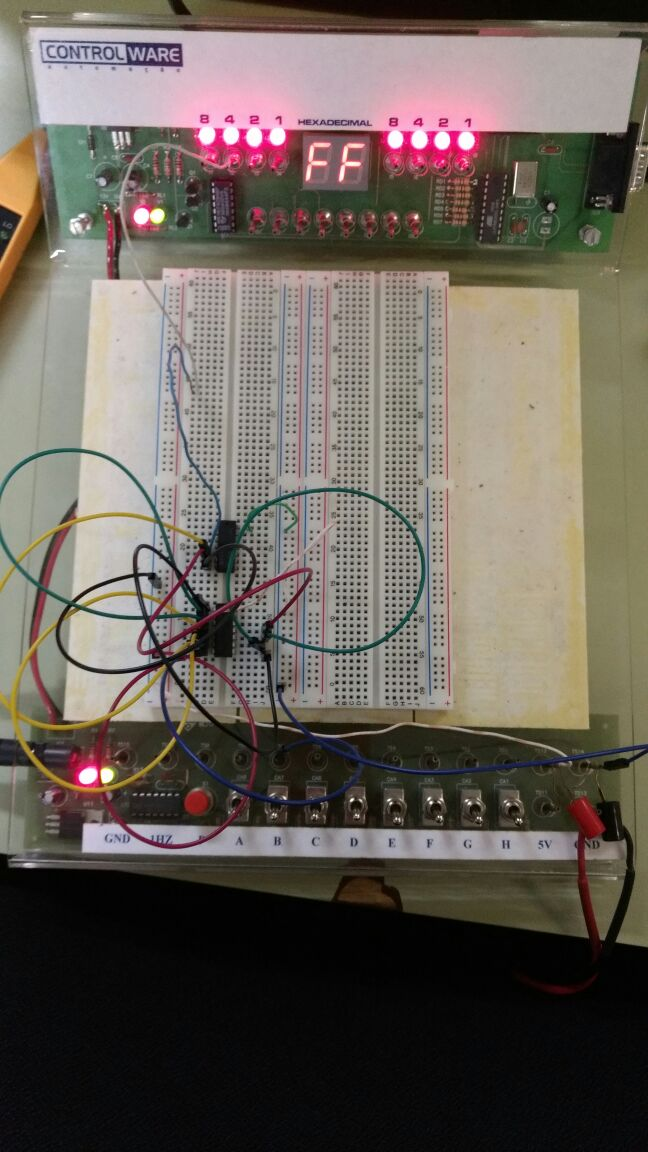
\includegraphics[width=.5\textwidth]{Porta_OR.jpeg}
\caption{Uma figura}
\label{fig:portaor}
\end{figure}

A Figura~\ref{fig:portaor} apresenta um exemplo de como usar e citar uma figura.

\begin{table}[H]
	\centering
	\begin{tabular}{|c|c|c|}
	\cline{1-3}
	\multicolumn{1}{|c|}{A} & \multicolumn{1}{|c|}{B} & \multicolumn{1}{|c|}{S1}\\
	\hline
	0 & 0 & 0 \\
	0 & 1 & 1 \\
	1 & 0 & 1 \\
	1 & 1 & 1 \\
	\hline
	\end{tabular}
	\label{ANDNOTOR}
\end{table}

\subsection{Implementação da porta AND com portas OR e NOT}
\label{sec:NOTOR}

\begin{figure}[H]
\centering
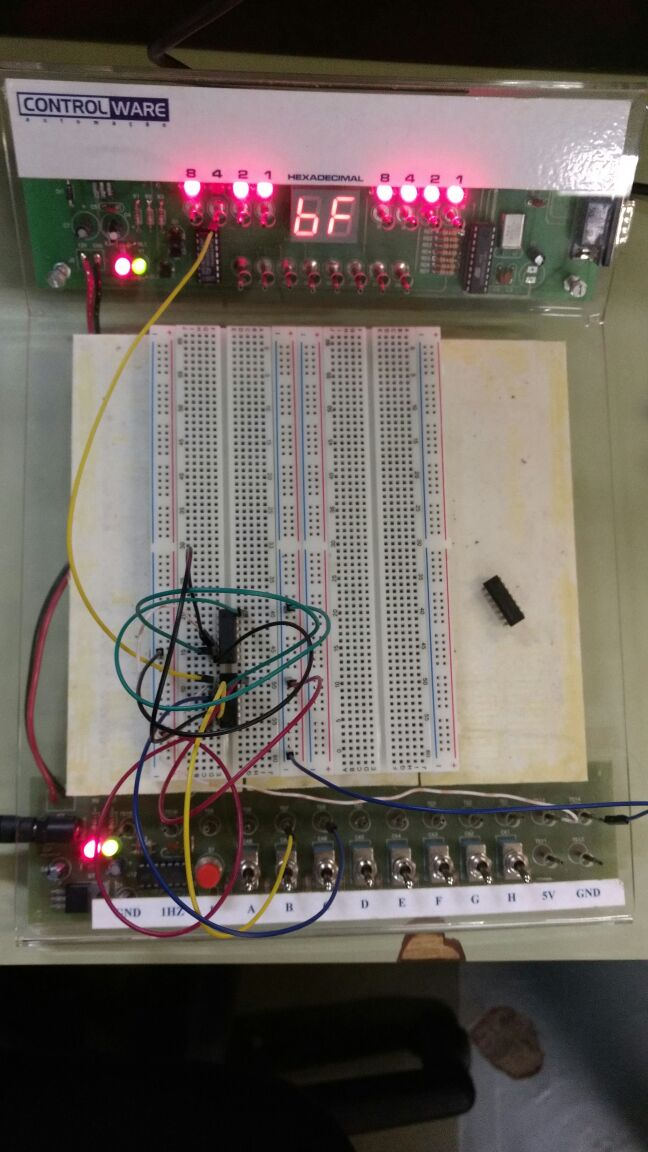
\includegraphics[width=.5\textwidth]{Porta_AND.jpeg}
\caption{Uma figura}
\label{fig:portaand}
\end{figure}

A Figura~\ref{fig:portaand} apresenta um exemplo de como usar e citar uma figura.

\begin{table}[H]
	\centering
	\begin{tabular}{|c|c|c|}
	\cline{1-3}
	\multicolumn{1}{|c|}{A} & \multicolumn{1}{|c|}{B} & \multicolumn{1}{|c|}{S1}\\
	\hline
	0 & 0 & 0\\
	0 & 1 & 0\\
	1 & 0 & 0\\
	1 & 1 & 1\\
	\hline
	\end{tabular}
	\label{ORNOTAND}
\end{table}

\subsection{Atraso de Propagação em Portas}
\label{sec:atraso}

Aqui temos um exemplo de como criar um hiperlink. Veja
\href{https://www.youtube.com/watch?v=EcNxjxKRQ6E}{aqui} um exemplo de vídeo.

Sempre identifique no site do vídeo:
\begin{itemize}
    \item o experimento: Experimento 7;
    \item semestre: 2016-2;
    \item a disciplina: CiC 116351 - Circuitos Digitais - Turma B;
    \item a universidade: Universidade de Brasília (UnB);
    \item os nomes dos componentes do grupo.
\end{itemize}

\section{Análise dos Resultados}
\label{sec:Resultados}


\section{Conclusão}
\label{sec:Conclusao}

Por este experimento obtivemos uma prática inicial com circuitos digitais, podemos nos familirializar com o protoboard e podemos por fim, compreender o atraso de propagação em portas  lógicas. 
Foi adquirido também um entendimento sobre as portas lógicas AND, NOT e OR, e que de fato, elas podem ser construídas de forma intercalada, determinando assim os conjuntos universais.


\bibliographystyle{sbc}
\bibliography{relatorio}


\newpage 
% Colocar aqui apenas as respostas dos itens da Auto-Avaliação
\section*{Auto-Avaliação}

\begin{enumerate}
    \item a
    \item c
    \item b
    \item d
\end{enumerate}


\end{document}
